\documentclass[tikz,border=5pt]{standalone}
\usepackage{amsmath}
\usepackage{graphicx}
\usetikzlibrary{arrows.meta,positioning,calc}

\definecolor{arrowgray}{HTML}{333333}
\definecolor{inputfill}{HTML}{EAF1F8}
\definecolor{inputborder}{HTML}{4A6B8A}
\definecolor{baselinefill}{HTML}{FBEBD9}
\definecolor{baselineborder}{HTML}{B8702E}
\definecolor{residualfill}{HTML}{E4F2E7}
\definecolor{residualborder}{HTML}{3C7A4A}
\definecolor{correctionfill}{HTML}{EDE4F5}
\definecolor{correctionborder}{HTML}{6A4C93}
\definecolor{predictionfill}{HTML}{E3EEF9}
\definecolor{predictionborder}{HTML}{2F5F8A}
\definecolor{evaluationfill}{HTML}{F2F2F2}
\definecolor{evaluationborder}{HTML}{7F7F7F}

\begin{document}
\resizebox{8.6cm}{!}{%
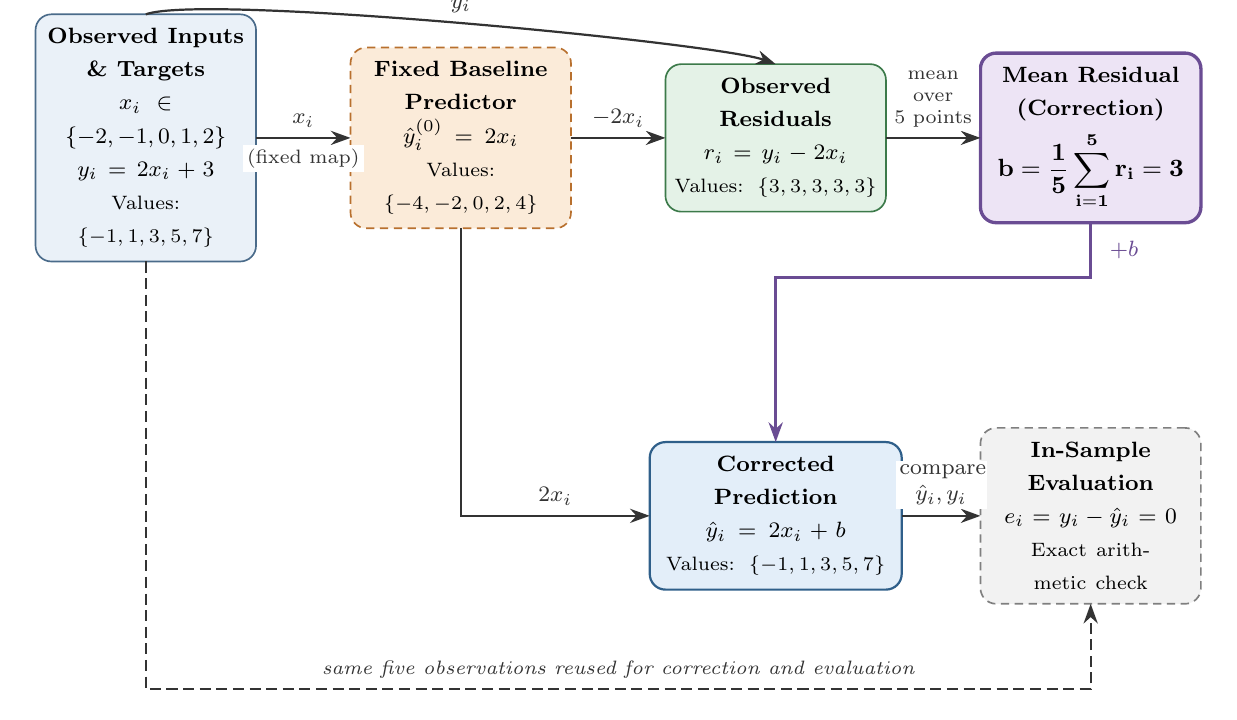
\begin{tikzpicture}[
    x=1cm,
    y=2cm,
    box/.style={
        rounded corners=2mm,
        line width=0.6pt,
        minimum height=1.4cm,
        align=center,
        text depth=0.25ex,
        text height=1.2ex,
        inner xsep=3pt,
        inner ysep=5pt,
        outer sep=0pt
    },
    multiline/.style={text height=,text depth=},
    flow/.style={
        -{Stealth[length=2.5mm,width=1.8mm]},
        line width=0.8pt,
        draw=arrowgray,
        rounded corners=0pt
    },
    labelbox/.style={
        align=center,
        inner sep=1.5pt,
        fill=white,
        text=arrowgray
    }
]

% A compact 16:9 drawing area; vertical coordinates are expanded
% to retain readable node proportions at single-column width.
\path[use as bounding box]
    (0.30,0.48125) rectangle (15.30,4.70);

\node[
    box,multiline,
    minimum width=2.8cm,
    minimum height=1.5cm,
    text width=2.58cm,
    fill=inputfill,
    draw=inputborder
] (inputs) at (1.8,4.0) {
    \textbf{\footnotesize Observed Inputs \& Targets}\\
    {\footnotesize $x_i\in\{-2,-1,0,1,2\}$}\\
    {\footnotesize $y_i=2x_i+3$}\\
    {\scriptsize Values: $\{-1,1,3,5,7\}$}
};

\node[
    box,multiline,
    minimum width=2.8cm,
    minimum height=1.5cm,
    text width=2.58cm,
    fill=baselinefill,
    draw=baselineborder,
    dash pattern=on 3pt off 2pt
] (baseline) at (5.8,4.0) {
    \textbf{\footnotesize Fixed Baseline Predictor}\\
    {\footnotesize $\hat{y}^{(0)}_i=2x_i$}\\
    {\scriptsize Values: $\{-4,-2,0,2,4\}$}
};

\node[
    box,multiline,
    minimum width=2.8cm,
    minimum height=1.5cm,
    text width=2.58cm,
    fill=residualfill,
    draw=residualborder
] (residuals) at (9.8,4.0) {
    \textbf{\footnotesize Observed Residuals}\\
    {\footnotesize $r_i=y_i-2x_i$}\\
    {\scriptsize Values: $\{3,3,3,3,3\}$}
};

\node[
    box,multiline,
    minimum width=2.8cm,
    minimum height=1.5cm,
    text width=2.58cm,
    fill=correctionfill,
    draw=correctionborder,
    line width=1.2pt
] (correction) at (13.8,4.0) {
    \textbf{\footnotesize Mean Residual (Correction)}\\[3pt]
    {\small $\displaystyle
        \mathbf{b=\frac{1}{5}\sum_{i=1}^{5}r_i=3}$}
};

\node[
    box,multiline,
    minimum width=3.2cm,
    minimum height=1.4cm,
    text width=2.98cm,
    fill=predictionfill,
    draw=predictionborder,
    line width=0.8pt
] (prediction) at (9.8,1.6) {
    \textbf{\footnotesize Corrected Prediction}\\
    {\footnotesize $\hat{y}_i=2x_i+b$}\\
    {\scriptsize Values: $\{-1,1,3,5,7\}$}
};

\node[
    box,multiline,
    minimum width=2.8cm,
    minimum height=1.4cm,
    text width=2.58cm,
    fill=evaluationfill,
    draw=evaluationborder,
    dash pattern=on 3pt off 2pt
] (evaluation) at (13.8,1.6) {
    \textbf{\footnotesize In-Sample Evaluation}\\
    {\footnotesize $e_i=y_i-\hat{y}_i=0$}\\
    {\scriptsize Exact arithmetic check}
};

\draw[flow]
    (inputs.east) --
    node[labelbox,above=2pt,font=\footnotesize] {$x_i$}
    node[labelbox,below=2pt,font=\scriptsize] {(fixed map)}
    (baseline.west);

\draw[flow]
    (inputs.north)
    to[out=20,in=160,looseness=0.25]
    node[labelbox,pos=0.5,above=2pt,font=\footnotesize] {$y_i$}
    (residuals.north);

\draw[flow]
    (baseline.east) --
    node[labelbox,above=2pt,font=\footnotesize] {$-2x_i$}
    (residuals.west);

\draw[flow]
    (residuals.east) --
    node[
        labelbox,
        above=2pt,
        font=\scriptsize,
        text width=1.05cm
    ] {mean over\\5 points}
    (correction.west);

\coordinate (baselinebend) at
    (baseline.south |- prediction.west);
\draw[flow]
    (baseline.south) --
    (baselinebend) --
    node[labelbox,above=2pt,font=\footnotesize] {$2x_i$}
    (prediction.west);

\coordinate (correctionbend) at
    ([yshift=-0.7cm]correction.south);
\draw[
    flow,
    draw=correctionborder,
    line width=1.2pt
]
    (correction.south) --
    node[
        right=3pt,
        text=correctionborder,
        font=\footnotesize\bfseries
    ] {$+b$}
    (correctionbend)
    -| (prediction.north);

\draw[flow]
    (prediction.east) --
    node[
        labelbox,
        above=2pt,
        font=\footnotesize,
        text width=1.05cm
    ] {compare\\$\hat{y}_i,y_i$}
    (evaluation.west);

\draw[
    flow,
    dash pattern=on 4pt off 2pt
]
    (inputs.south) --
    (1.8,0.5) --
    node[
        labelbox,
        midway,
        above=2pt,
        font=\scriptsize\itshape
    ] {same five observations reused for correction and evaluation}
    (13.8,0.5) --
    (evaluation.south);

\end{tikzpicture}%
}
\end{document}